\section*{Actividad 2}

Para aproximarnos al problema de la princesa Dido desde la optimización, podemos imaginar una elipse, cuyos semiejes denominaremos $a$ y $b$.

\begin{center}
    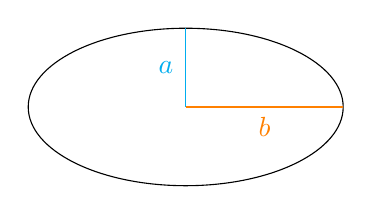
\begin{tikzpicture}
        \draw (0,0) ellipse (2cm and 1cm);
        \draw[-, cyan] (0,0) -- (0,1); % línea a
        \draw[cyan] (-0.25,0.5) node{$a$}; % label a
        \draw[-, orange] (0,0) -- (2,0); % línea b
        \draw[orange] (1,-0.25) node{$b$}; % label b
    \end{tikzpicture}
\end{center}

Podemos plantear dos ecuaciones, una para su área:

\begin{align*}
    A &= \pi ab
\end{align*}

Y otra para su perímetro:

\begin{align*}
    P &= \pi (a + b)
\end{align*}

En nuestro caso, el perímetro funciona como una restricción, a partir de la cual podemos despejar $a$, para expresar el área del elipse en función de $b$:

\begin{align*}
    \pi (a + b) &= 100\\
    a &= \frac{100}{\pi} - b
\end{align*}

Expresamos el área en función de $b$:

\begin{align*}
    A &= \pi b (\frac{100}{\pi} - b)\\
    A &= 100b - \pi b^2
\end{align*}

Derivamos esta función:

\begin{align*}
    \frac{dA}{dx} &= 100 - 2 \pi b
\end{align*}

E igualamos a 0, para determinar el punto máximo de la función del área:

\begin{align*}
    100 - 2 \pi b &= 0\\
    b &= \frac{-100}{-2 \pi}\\
    b &= \frac{50}{\pi}
\end{align*}

De ahí determinamos que $a$ es: 

\begin{align*}
    a &= \frac{100}{\pi} - \frac{50}{\pi}\\
    a &= \frac{50}{\pi}\\
    a &= b
\end{align*}

La elipse cuyos semiejes son iguales, en este caso $a$ y $b$, es el círculo. El círculo sería entonces la figura que maximizaría el área.
